\chapter{Maschinelles Lernen}
Das maschinelle Lernen ist ein Teilgebiet der künstlichen Intelligenz und übernimmt Aufgaben die typischerweise menschliche Intelligenz erfordern. Sie soll dabei helfen Muster und Gesetzmäßigkeiten in Datensätzen zu erkennen. Aus vorhandenen Daten wird durch Algorithmen künstliches Wissen generiert.

\section{Methoden maschinellen Lernens}
Maschinelles Lernen lässt sich nach [\href{https://www.talend.com/de/resources/maschinelles-lernen}{talend.com}] in vier Methoden unterteilen. Die in den folgenden Kapiteln näher betrachtet werden.

\subsection{Überwachtes Lernen}
Bei überwachtem Lernen erhält ein Computer strukturierte Inputs und gewünschte Ergebnisse. Nun muss der Computer Wege finden mit Inputs, um diese Ergebnisse zu erreichen, d.h der Algorithmus versucht eine vorhersage Funktion zu entwickeln. Die Vorhersagen über die unbekannten oder künftigen Daten wird als prädiktive Modellierung bezeichnet.\vspace{0.2cm}

Das überwachte Lernen lässt sich in zwei Arten unterteilen.
\begin{itemize}
	\item Klassifizierung: das Ergebnis ist eine Kategorie, z. B. Gruppenzugehörigkeit
	\item Regression: hier ist das Ergebnis ein realer Wert, z. B. Produktpreis
\end{itemize}

Mittels verschiedener Methoden lassen sich die Ergebnisse vorhersagen. Diese können Entscheidungsbäume, Random-Forest-Algorithmus, lineare Regression, Naive-Bayes-Verfahren, usw. Eignet sich für Probleme der Klassifizierung und Regression.

\subsection{Unüberwachtes Lernen}
Bei diesem Lernen sind keine strukturieren Daten vorhanden, eher legen sie unstrukturiert und unbeschriftet vor. Der Algorithmus muss die Strukturen selbst erkennen. Aus erkannten Mustern und Merkmalen, lassen sich weitere Muster und Korrelationen vorhersagen. Ist, gibt zwei Arten von unüberwachten Lernen.
\begin{itemize}
	\item Clustering: Gruppierung von Daten, weitere lassen sich in bestehende Cluster zuordnen
	\item Assoziation: Regeln in Daten finden, so werden Daten durch Erfahrung definiert
\end{itemize}

Zu diesem Lernen gehören u. a. K-Means, hierarchische Clusteranalyse und Dimensionsreduktion. Mit dieser Methode lassen sich Probleme des Clustering, Dimensionsreduktion und Lernen von Assoziationsregeln.

\subsection{Teilweise überwachtes Lernen}
Es ist ein Hybridverfahren zwischen unüberwachten und überwachten Lernen. Die Rohdaten sind nur teilweise strukturiert und beschriftet. Durch die strukturierten Daten werden die unstrukturierten aufgewertet.\vspace{0.2cm}

Die strukturierten Daten finden anfangs Verwendung, um diese auf Muster und Korrelationen zu untersuchen. Im Anschluss können diese auf die unstrukturierten angewandt werden. Mit dem teilweise überwachten Lernen können Probleme der Klassifizierung und Regression gelöst werden.

\subsection{Bestärktes Lernen}
Ein Computerprogramm interagiert mit einer dynamischen Umgebung. Beim Ausführen bestimmter Aufgaben erhält das Programm gutes oder schlechtes Feedback für die Aktion. Durch die Belohnung und Bestrafung lernt das Programm die richtigen Verhaltensweisen. Belohnungen werden auf zwei verschiedene Arten vergeben.

\begin{itemize}
	\item Monte Carlo: Vergabe erfolgt am Ende
	\item Temporal-Difference-Learning (TD-Learning): Vergabe der Belohnung erfolgt nach jedem Schritt
\end{itemize}

Als Algorithmen sind hier beispielsweise Q-Learning, Deep Q Network (DQN) und State-Action-Reward-State-Action (SARSA) zu nennen.

\section{Algorithmen zum Analysieren von Onlineshop Daten}
Für die Ermittlung der Klassifizierung werden Daten verwendet, bei denen ein Nutzer einen Kauf abgeschlossen hat. Die folgenden Daten werden berücksichtigt,
\begin{itemize}
	\item 
	\item Warenkorbhöhe
	\item Gekauften Artikel pro Warenkorb
	\item Anzahl der zuvor besuchten Seiten
	\item Einstiegsseite
	\item Datum
\end{itemize}
Diese Daten werden im FP-Growth-Algorithmus und mittels neuronalen Netzwerk ausgewertet und im Anschluss verglichen.

\subsection{FP-Growth-Algorithmus}
FP-Growth steht für Frequent Pattern (deutsch: häufige Muster). Er ist eine Verbesserung des Apriori Algorithmus da und stellt die Daten in einer Baumstruktur dar, mit den häufigsten Muster. Dabei repräsentiert jedes Blatt des Baumes ein Item eines Itemsets.\vspace{0.2cm}

Der FP-Growth ist ein schnell arbeitender Algorithmus, der gut skalieren ist und auch versteckte Muster in Datensätzen findet. Der Algorithmus arbeitet effizienter als beispielsweise der Apriori Algorithmus oder die TreeProjection.\vspace{0.2cm}

Der Nachteil dieses Algorithmus ist, dass er sehr komplex ist und für kleine Datenmengen Algorithmen wie beispielsweise der bereits genannte Apriori Algorithmus ausreicht.\vspace{0.2cm}

Dieser Algorithmus wird unter anderem von Apache Spark [\href{https://spark.apache.org/docs/latest/ml-frequent-pattern-mining.html}{1}] eingesetzt.

\subsection{Neuronales Netz}
Bei neuronalen Netzen handelt es sich um dem Nervensystem nachempfundenes Netz. Die Idee stammt aus der Neurobiologie und soll die Signale weiterleiten. Dadurch soll ein neuronales Netz in die Lage versetzt werden abstrakte Konzepte zu erlernen. Die Übermittlung der Signale von einem Neuron zum nächsten kann bei künstlicher Intelligenz nur bei trainierten Netzen erfolgen.

\subsubsection{Einsatzzwecke für neuronale Netze}
Prinzipiell gibt es drei Hauptanwendungen für neuronale Netze. Die Abbildung \ref{img:types_of_ml} zeigt deren Verwendungszwecke.\vspace{0.2cm}

\begin{figure}[!ht]
	\centering
	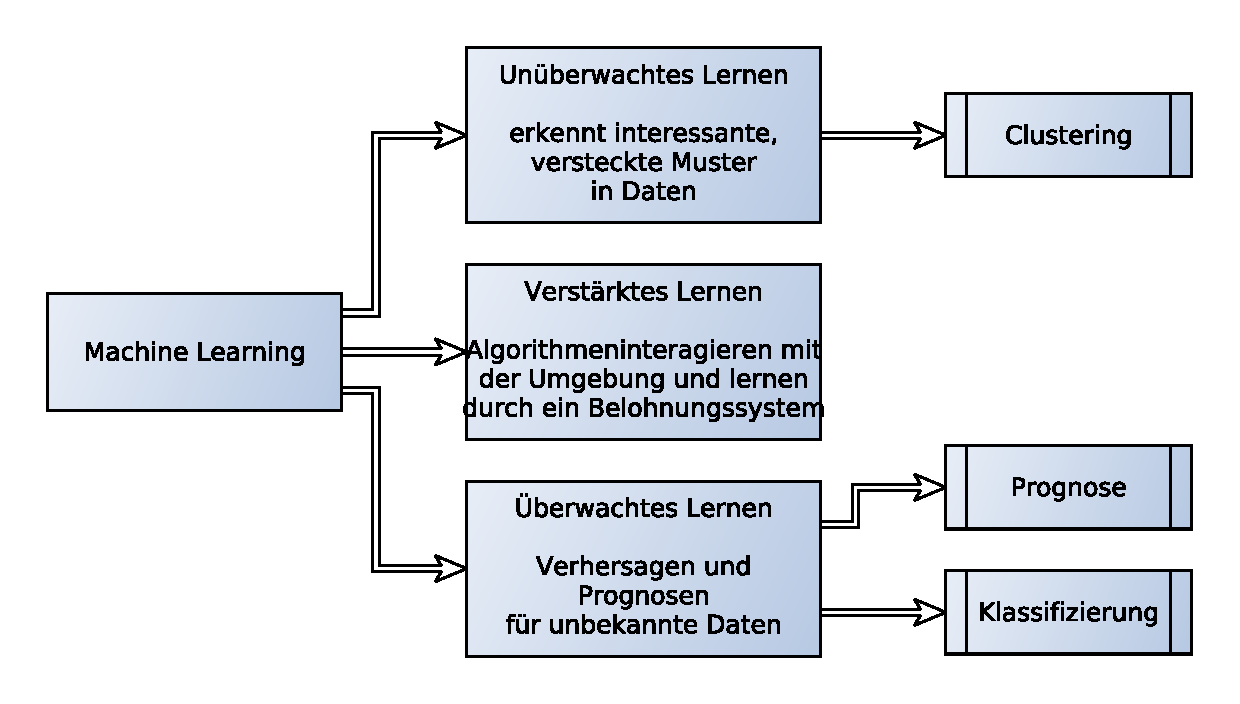
\includegraphics[width=\linewidth]{images/chapter5/ml_types.eps}
	\caption{Übersicht zu neuronalen Netzen und ihrer Verwendung}
	\label{img:types_of_ml}
\end{figure}

\textit{Classification (Supervised Machine Learning)} das Netz wird mit Trainingsdaten trainiert und berechnet für neue Datensätze die Kategorie, in der die Informationen eines Datensatzes passen.\vspace{0.2cm}

\textit{Regiession (Supervised Machine Learning)} ähnlich wie bei der Classification werden diese Netze trainiert, um Vorhersagen zu treffen. Beispielsweise für optimale Preise, Retouren und Umsatzzahlen.\vspace{0.2cm}

\textit{Clustering (Unsupervised Machine Learning)} erkennt Gruppen anhand ähnlicher Merkmale. Diese Netze benötigen kein Training, da nur die reinen Informationen innerhalb der Datensätze nutzen, um Muster zuerkennen.

\subsubsection{Arten von neuronalen Netzen}
\textit{Perception} sind die einfachsten Netze. Sie bestehen nur aus einem Input-Layer und einer Aktivierungsfunktion im Output-Layer. Hidden-Layer gibt es hierbei nicht.\vspace{0.2cm}

\textit{Feedforward artificial neural network (FFNN)} hierbei bewegen sich die Signale in eine Richtung. Diese Netze besitzen aber auch Hidden-Layer.\vspace{0.2cm}

\textit{Deep Learning (DL)} diese Netze besitzen mehrere Hidden-Layer Schichten.\vspace{0.2cm}

\textit{Recurrent neural networks (RNN)} betrachten, im Vergleich zu den FFNN Netzen auch temporäre Sequenzen, indem sie Informationen zwischenspeichern. Sie gelten deshalb als einer der stärksten neuronalen Netze.\vspace{0.2cm}

\textit{Symmetrically connected neural network} sind aufgebaut wie RNN’s haben aber eine symmetrische Topologie in der Anordnung und Zuweisung der Gewichte.\vspace{0.2cm}

\textit{Convoluted neural networks (CNN)} diese Netze betrachten die Signale nicht linear, sondern betrachte regionale Signale. Dadurch werden Ergebnisse genauer und das Training wird schneller und effizienter.\vspace{0.2cm}

\textit{Radial basis function network (RBFN)} sind einfache FFNN Netzwerke die aber die Distanz zwischen den Knoten miteinbeziehen.\vspace{0.2cm}

\textit{Self organizing neural network} finden Verwendung, um Strukturen innerhalb von Datensätzen zu finden. Diese Netze arbeiten unsupervised.
Moduar neural network kombinieren mehrere neurale Netzwerke, um verschiedene Teilaufgaben zu lösen.\vspace{0.2cm}

\textit{Generative adversarial networks (GAN)} generieren aus den zu lernenden Daten neue Daten. Hier werden zwei Netze kombiniert. Ein Netz generiert Daten das andere Netz überprüft diese.

\subsubsection{Aufbau des neuronalen Netzes}
In dieser Arbeit wird das Feedforward artificial neural network (FFNN) verwendet. Die einzelnen Nervenzellen werden hierbei als Neuronen bezeichnet und sind Funktionen die auf Basis des Inputs und der Gewichtung den Output berechnen. Die Schichten auf denen die Neuronen liegen als Layer. Bei den Layern gibt die Input-Layer, den oder die Hidden-Layer und den Output-Layer. Die Neuronen der einzelnen Layer sind mit Kanten untereinander verbunden, welche mit Gewichtungen, die Ausgaben für das nächste Neuron umrechnet.
\subsubsection{Training neuronaler Netze}
Zuerst erfolgt die Übergabe der Kundenattribute an die Input-Neuronen. Die Attribute enthalten die Bestelldaten, Daten zum Nutzerverhalten und zusätzlichen externen Daten.\vspace{0.2cm}

Zunächst wird das Netz trainiert. Die Initialisierung der Gewichtig muss gut überlegt sein, da es sonst dazu führen kann, das das Netz langsam lernt oder alle Hidden-Layer das gleiche lernen. Nur wird das Netz mit dem Input geladen und iterativ werden die Gewichte der Kanten definiert. Die Signale werden durch die Layer zum Output-Layer geleitet, also zum Ende hin. Dieses Verfahren wird auch als Forward Propagation bezeichnet. Hier sei noch einmal auf die Datenqualität hingewiesen. Ist die Datenqualität schlecht oder stehen nicht genügend Daten zur Verfügung kann das nicht oder schlecht trainiert werden. Sind die Signale am Output-Layer angekommen, definieren Aktivierungsfunktionen (eng. Activation Function), ob das Netz feuert oder nicht.\vspace{0.2cm}

Nun wird der Output des neuronalen Netzes mit den vorher definierten Ausgaben. Bei einer Abweichung wird dann rückwärts durch das Netz propagiert (eng. Back Propagation) und das Netz lernt daraus. D. h. die Gewichte werden angepasst. Der Vorgang des Inputs laden, Fehler berechnen und Gewichte korrigieren, wird so lange wiederholt, bis ein festgelegtes Abbruchkriterium greift. Nun ist das Netz trainiert.

\section{Umsetzung der Datenverarbeitung}
%So was wie Daten bereinigen und zusammenführen.
Erste Tests in Sachen Python und Datenanalyse. Kommt ein Kapitel früher.

\begin{figure}[!ht]
	\centering
	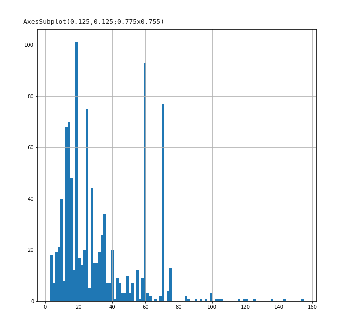
\includegraphics[width=\linewidth]{images/chapter4/first_plot.eps}
	\caption{Anzahl der Bestellung in Abhängigkeit der Warenkorbhöhe}
	\label{img:plot_count_amount}
\end{figure}

\section{Umsetzung ds FP-Grwoth-Algorithmus}
Zur Analyse der zusammen verkauften Artikel und Assoziationsregeln zum Nutzerverhalten aufstellen zu können und einen Merkmals-Vektor zu erstellen, um auf dessen Grundlage die Benutzerklassifizierung zu ermitteln.\vspace{0.2cm}

Im ersten Schritt werden alle vorbereiteten Datensätze durchlaufen, um die Anzahl der Items zu finden, die für die Klassifizierung der Nutzer erforderlich ist. Im Anschluss werden alle Items erfasst, die den minimalen Support erfüllen. Anschließend werden die Datensätze wiederholt durchsucht und nach den minimalen Support-Items gesucht.\vspace{0.2cm}

Daraus wird der Häufigkeitsbaum erstellt, in dem alle Items und Datensätze abgebildet werden.

\section{Umsetzung mittels neuronalen Netz}
